% This is "sig-alternate.tex" V2.1 April 2013
% This file should be compiled with V2.5 of "sig-alternate.cls" May 2012
%
% This example file demonstrates the use of the 'sig-alternate.cls'
% V2.5 LaTeX2e document class file. It is for those submitting
% articles to ACM Conference Proceedings WHO DO NOT WISH TO
% STRICTLY ADHERE TO THE SIGS (PUBS-BOARD-ENDORSED) STYLE.
% The 'sig-alternate.cls' file will produce a similar-looking,
% albeit, 'tighter' paper resulting in, invariably, fewer pages.
%
% ----------------------------------------------------------------------------------------------------------------
% This .tex file (and associated .cls V2.5) produces:
%       1) The Permission Statement
%       2) The Conference (location) Info information
%       3) The Copyright Line with ACM data
%       4) NO page numbers
%
% as against the acm_proc_article-sp.cls file which
% DOES NOT produce 1) thru' 3) above.
%
% Using 'sig-alternate.cls' you have control, however, from within
% the source .tex file, over both the CopyrightYear
% (defaulted to 200X) and the ACM Copyright Data
% (defaulted to X-XXXXX-XX-X/XX/XX).
% e.g.
% \CopyrightYear{2007} will cause 2007 to appear in the copyright line.
% \crdata{0-12345-67-8/90/12} will cause 0-12345-67-8/90/12 to appear in the copyright line.
%
% ---------------------------------------------------------------------------------------------------------------
% This .tex source is an example which *does* use
% the .bib file (from which the .bbl file % is produced).
% REMEMBER HOWEVER: After having produced the .bbl file,
% and prior to final submission, you *NEED* to 'insert'
% your .bbl file into your source .tex file so as to provide
% ONE 'self-contained' source file.
%
% ================= IF YOU HAVE QUESTIONS =======================
% Questions regarding the SIGS styles, SIGS policies and
% procedures, Conferences etc. should be sent to
% Adrienne Griscti (griscti@acm.org)
%
% Technical questions _only_ to
% Gerald Murray (murray@hq.acm.org)
% ===============================================================
%
% For tracking purposes - this is V2.0 - May 2012

\documentclass{sig-alternate-05-2015}
\usepackage{epstopdf}
\usepackage[nomain, acronym, toc]{glossaries}
\usepackage{pgfplots}

\setlength{\arrayrulewidth}{0.2pt}%.4pt
{\renewcommand{\arraystretch}{1.2}

\definecolor{rosso}{RGB}{220,57,18}
\definecolor{giallo}{RGB}{255,153,0}
\definecolor{blu}{RGB}{102,140,217}
\definecolor{verde}{RGB}{16,150,24}
\definecolor{viola}{RGB}{153,0,153}

\makeatletter

\tikzstyle{chart}=[
    legend label/.style={font={\scriptsize},anchor=west,align=left},
    legend box/.style={rectangle, draw, minimum size=5pt},
    axis/.style={black,semithick,->},
    axis label/.style={anchor=east,font={\tiny}},
]

\tikzstyle{bar chart}=[
    chart,
    bar width/.code={
        \pgfmathparse{##1/2}
        \global\let\bar@w\pgfmathresult
    },
    bar/.style={very thick, draw=white},
    bar label/.style={font={\bf\small},anchor=north},
    bar value/.style={font={\footnotesize}},
    bar width=.75,
]

\tikzstyle{pie chart}=[
    chart,
    slice/.style={line cap=round, line join=round, very thick,draw=white},
    pie title/.style={font={\bf}},
    slice type/.style 2 args={
        ##1/.style={fill=##2},
        values of ##1/.style={}
    }
]

\pgfdeclarelayer{background}
\pgfdeclarelayer{foreground}
\pgfsetlayers{background,main,foreground}


\newcommand{\pie}[3][]{
    \begin{scope}[#1]
    \pgfmathsetmacro{\curA}{90}
    \pgfmathsetmacro{\r}{1}
    \def\c{(0,0)}
    \node[pie title] at (90:1.3) {#2};
    \foreach \v/\s in{#3}{
        \pgfmathsetmacro{\deltaA}{\v/100*360}
        \pgfmathsetmacro{\nextA}{\curA + \deltaA}
        \pgfmathsetmacro{\midA}{(\curA+\nextA)/2}

        \path[slice,\s] \c
            -- +(\curA:\r)
            arc (\curA:\nextA:\r)
            -- cycle;
        \pgfmathsetmacro{\d}{max((\deltaA * -(.5/50) + 1) , .5)}

        \begin{pgfonlayer}{foreground}
        \path \c -- node[pos=\d,pie values,values of \s]{$\v\%$} +(\midA:\r);
        \end{pgfonlayer}

        \global\let\curA\nextA
    }
    \end{scope}
}

\newcommand{\legend}[2][]{
    \begin{scope}[#1]
    \path
        \foreach \n/\s in {#2}
            {
                  ++(0,-10pt) node[\s,legend box] {} +(5pt,0) node[legend label] {\n}
            }
    ;
    \end{scope}
}

% Acronym Definition

\newacronym{IST}{IST}{Instituto Superior T\'ecnico}
\newacronym{IoT}{IoT}{Internet of Things}
\newacronym{MQTT}{MQTT}{Message Queue Telemetry Transport}
\newacronym{MQTT-SN}{MQTT-SN}{Message Queue Telemetry Transport for Sensor Networks}
\newacronym{CoAP}{CoAP}{Constrained Application Protocol}
\newacronym{HTTP}{HTTP}{Hypertext Transfer Protocol}
\newacronym{TLS}{TLS}{Transport Layer Security}
\newacronym{DTLS}{DTLS}{Datagram Transport Layer Security}
\newacronym{WWW}{WWW}{World Wide Web}
\newacronym{MTU}{MTU}{Maximum Transmission Unit}
\newacronym{TCP}{TCP}{Transmission Control Protocol}
\newacronym{REST}{REST}{REpresentational State Transfer}
\newacronym{UDP}{UDP}{User Datagram Protocol}
\newacronym{URIs}{URIs}{Universal Resource Identifiers}
\newacronym{M2M}{M2M}{Machine to Machine}
\newacronym{QoS}{QoS}{Quality of Service}
\newacronym{WLAN}{WLAN}{Wireless Local Area Networks}
\newacronym{WPAN}{WPAN}{Wireless Private Area Networks}
\newacronym{LR-WPAN}{LR-WPAN}{Low-Rate Wireless Private Area Networks}
\newacronym{MAC}{MAC}{Medium Access Control}
\newacronym{FFD}{FFD}{Full Function Device}
\newacronym{RFD}{RFD}{Reduced Function Device}
\newacronym{IETF}{IETF}{Internet Engineering Task Force}
\newacronym{DoS}{DoS}{Denial of Service}
\newacronym{DODAG}{DODAG}{Destination Oriented Directed Acyclic Graph}
\newacronym{DIO}{DIO}{DODAG Information Objects}
\newacronym{DAO}{DAO}{Destination Advertisement Objects}
\newacronym{DIS}{DIS}{DODAG Information Solicitation}
\newacronym{RFID}{RFID}{Radio Frequency Identification}
\newacronym{ACL}{ACL}{Access Control List}
\newacronym{6LoWPAN}{6LoWPAN}{IPv6 over Low power Wireless Personal Area Networks}
\newacronym{RPL}{RPL}{Routing Protocol for Low-Power and Lossy Networks}
\newacronym{CA}{CA}{Certificate Authority}
\newacronym{CSDS}{CSDS}{\gls{CoAP} Service Discovery Server}
\newacronym{RDC}{RDC}{Radio Duty Cycling}

\begin{document}

% Copyright
\setcopyright{acmcopyright}
%\setcopyright{acmlicensed}
%\setcopyright{rightsretained}
%\setcopyright{usgov}
%\setcopyright{usgovmixed}
%\setcopyright{cagov}
%\setcopyright{cagovmixed}


% DOI
\doi{10.475/123_4}

% ISBN
\isbn{123-4567-24-567/08/06}

%Conference
\conferenceinfo{PLDI '13}{June 16--19, 2013, Seattle, WA, USA}

\acmPrice{\$15.00}

%
% --- Author Metadata here ---
\conferenceinfo{ACSAC}{'16 Los Angeles, California USA}
%\CopyrightYear{2007} % Allows default copyright year (20XX) to be over-ridden - IF NEED BE.
%\crdata{0-12345-67-8/90/01}  % Allows default copyright data (0-89791-88-6/97/05) to be over-ridden - IF NEED BE.
% --- End of Author Metadata ---

%\title{Securing Smart Places: A Power-Aware Infrastructure}
\title{Attack Prevention on IoT Environments by\\ Secure Bootstrapping 6LoWPAN Networks}
%
% You need the command \numberofauthors to handle the 'placement
% and alignment' of the authors beneath the title.
%
% For aesthetic reasons, we recommend 'three authors at a time'
% i.e. three 'name/affiliation blocks' be placed beneath the title.
%
% NOTE: You are NOT restricted in how many 'rows' of
% "name/affiliations" may appear. We just ask that you restrict
% the number of 'columns' to three.
%
% Because of the available 'opening page real-estate'
% we ask you to refrain from putting more than six authors
% (two rows with three columns) beneath the article title.
% More than six makes the first-page appear very cluttered indeed.
%
% Use the \alignauthor commands to handle the names
% and affiliations for an 'aesthetic maximum' of six authors.
% Add names, affiliations, addresses for
% the seventh etc. author(s) as the argument for the
% \additionalauthors command.
% These 'additional authors' will be output/set for you
% without further effort on your part as the last section in
% the body of your article BEFORE References or any Appendices.

\numberofauthors{2} %  in this sample file, there are a *total*
% of EIGHT authors. SIX appear on the 'first-page' (for formatting
% reasons) and the remaining two appear in the \additionalauthors section.
%
\author{
% You can go ahead and credit any number of authors here,
% e.g. one 'row of three' or two rows (consisting of one row of three
% and a second row of one, two or three).
%
% The command \alignauthor (no curly braces needed) should
% precede each author name, affiliation/snail-mail address and
% e-mail address. Additionally, tag each line of
% affiliation/address with \affaddr, and tag the
% e-mail address with \email.
%
% 1st. author
\alignauthor
Tiago Diogo\\
       \affaddr{Instituto Superior Técnico}\\
       \affaddr{Av. Rovisco Pais, 1}\\
       \affaddr{1049-001 Lisboa, Portugal}\\
       \email{tiago.diogo@tecnico.ulisboa.pt}
% 2nd. author
\alignauthor
Miguel Pardal\\
       \affaddr{Instituto Superior Técnico}\\
       \affaddr{Av. Rovisco Pais, 1}\\
       \affaddr{1049-001 Lisboa, Portugal}\\
       \email{miguel.pardal@tecnico.ulisboa.pt}
}
% There's nothing stopping you putting the seventh, eighth, etc.
% author on the opening page (as the 'third row') but we ask,
% for aesthetic reasons that you place these 'additional authors'
% in the \additional authors block, viz.

% Just remember to make sure that the TOTAL number of authors
% is the number that will appear on the first page PLUS the
% number that will appear in the \additionalauthors section.

\maketitle
\begin{abstract}
The \gls{IoT} and its vision of connecting devices to one another and to the Internet presents an opportunity to create large information sharing networks. However, intruders can capture and take advantage of the \gls{IoT} devices constrained nature to disrupt these networks and launch a wide range of attacks on its nodes.
In our work we propose a secure bootstrapping infrastructure capable of securing \gls{IoT} environments based on 6LoWPAN networks. To achieve this, we do a thorough analysis of the existing protocols, attacks and mitigation strategies, combining that information into our proposed network management system.
Furthermore, we measure the space and energy required for operation in order to assess what kind of physical resources to deploy, based on the network security characteristics.
\end{abstract}


%
% The code below should be generated by the tool at
% http://dl.acm.org/ccs.cfm
% Please copy and paste the code instead of the example below. 
%
\begin{CCSXML}
<ccs2012>
<concept>
<concept_id>10010520.10010553.10003238</concept_id>
<concept_desc>Computer systems organization~Sensor networks</concept_desc>
<concept_significance>500</concept_significance>
</concept>
<concept>
<concept_id>10002978.10003014.10003017</concept_id>
<concept_desc>Security and privacy~Mobile and wireless security</concept_desc>
<concept_significance>300</concept_significance>
</concept>
</ccs2012>  
\end{CCSXML}

\ccsdesc[500]{Computer systems organization~Sensor networks}
\ccsdesc[300]{Security and privacy~Mobile and wireless security}


%
% End generated code
%

%
%  Use this command to print the description
%
\printccsdesc

% We no longer use \terms command
%\terms{Theory}

\keywords{Internet of Things; Power-Aware Security; Secure Bootstrapping; CoAP; 6LoWPAN; RPL; IEEE 802.15.4}

\section{Introduction}
The Internet of Things can be seen as a web of interconnected devices that range from everyday wearable objects to enterprise grade sensor networks. Despite the huge variety and characteristics of these devices, one characteristic that they all have in common is their constrained nature. In order to enable the massive deployment to be expected in the near future, \gls{IoT} devices must be accessible and affordable, capable of operating under lossy wireless networks while being battery powered. Section \ref{sec:network_overview} presents an overview of the type of networks and scenarios under consideration. Since \gls{IoT} environments can range from home to enterprise or even city environments, a breach in security could potentially leak important core company activity or provide information about individuals choices and whereabouts constituting a violation of privacy \cite{Ukil2015}. To this extent a study on existing attacks for constrained devices was conducted in Section \ref{sec:attack_analysis} and a common mitigation strategy (secure bootstrapping) presented in Section \ref{sec:secure_bootstrapping}. This strategy provided security assurances at the cost of an increased infrastructure complexity, which in its turn created the necessity for a management station capable of storing and writing network credentials onto new nodes. Our proposed system architecture is presented in Section \ref{sec:system_architecture} and some implementation details are given in Section \ref{sec:implementation_details}. In order to accurately define the type and amount of resources needed to create such a network, we deployed our protocol stack and management station on physical hardware and performed space and power measurements as presented in Section \ref{sec:evaluation}. Finally, Section \ref{sec:conclusion} states our conclusions and opportunities for future work.

\section{Environment Overview}
\label{sec:network_overview}
There are many applicability domains and different methods for creating \gls{IoT} networks. Some provide direct connectivity of nodes to the Internet while others provide a common gateway for interfacing with external networks. In our work, we focus on scenarios where network nodes are not directly connected to the internet and require additional network components for proper communication as depicted in Figure \ref{fig:net_overview}.
In this type of architectures, the sensing or actuating nodes belong to a very constrained network with specific protocols and header compression mechanisms, requiring an interface device, the border router, in order to communicate with external networks. After reaching the external network, incoming messages are processed to convert sensor data into useful information being then stored or used to trigger events. This information can then be consulted by users either on the same network or by making requests through the Internet. This type of infrastructures could be used for example in a home intrusion system or in a factory monitoring system. In the home intrusion system scenario, the network nodes would create a sensor network that propagates events in the case of an intrusion and the additional infrastructure would be in charge of receiving these events and notifying the authorities. In the factory monitoring system scenario, the network nodes would create a sensor network that would be permanently reporting up to date values of machinery control values like temperature, pressure and power and the additional infrastructure would in charge of supplying this information to a dashboard for the factory workers. If an attacker could disable these systems, he could then rob the house or cause an emergency shut-down of the factory machinery due to lack of control over the working conditions. These are real concerns backed by a breed of attacks that focuses on disabling \gls{IoT} networks by placing the nodes offline. These attacks are presented in the following section.

\begin{figure}[h]
  \centering
  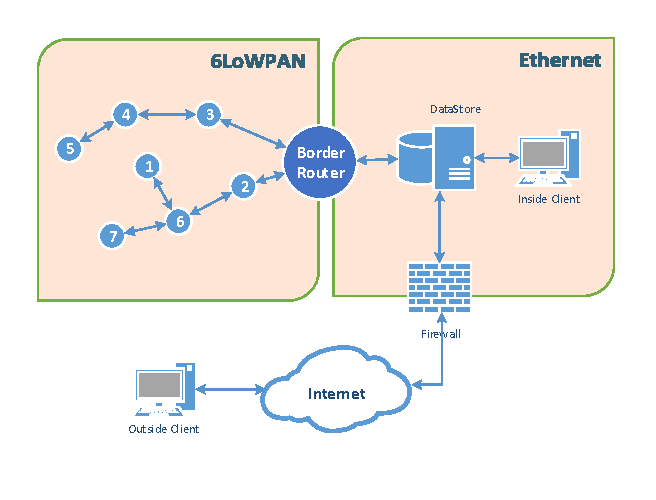
\includegraphics[width=1.0\linewidth]{figures/Network_Overview.pdf}
  \caption{Network Overview}
  \label{fig:net_overview}
\end{figure}

\section{Attack Analysis}
\label{sec:attack_analysis}
Exploitation of existing solutions in the forms of malicious attacks can be found at all the studied OSI layers. They can go from a physical intruder replacing some node on a sensor field to the well-known \gls{DoS} at the application layer. However, given the characteristics of the devices and networks used in \gls{IoT} combined with the power consumption focus of this work, a specific kind of attacks performed at the network layer is of special interest and importance: battery depletion attacks, also known as, ``vampire'' attacks.

Battery depletion attacks aim at draining the battery, ``life'', of the network devices, working over time to entirely disable a network, hence being called ``vampire'' attacks. These attacks do not focus on flooding the network with many packages, instead they drain the node's life by delaying the packets transmission. Some of them target specific implementations while others are protocol independent \cite{Vasserman2013}\cite{Pongle2015}. In the following paragraphs, we present a couple of attacks, performed on different routing solutions that demonstrate the draining power of these attacking methods.

\subsection{Stateless Protocols}
\label{sec:source_routing}
In systems that use this type of routing protocols, the source node specifies the entire route to the destination in the packet header. This means that intermediaries do not make decisions regarding the next hop, they only forward to the next node as specified in the original path therefore reducing the amount of computation performed and used energy. Using this transmission scheme, a malicious device can specify paths through the network that are far from optimal, wasting energy at the intermediate nodes who follow the included malicious source route. The Carousel Attack is an example of such attacks. Its objective is to send a packet along a route composed as a series of loops. This way, a single node may forward the malicious packet several times increasing the total energy consumption by a factor of the number of loops the attacker has introduced on the packet header path. It targets source routing protocols by exploiting the limited verification of the packet headers at the intermediary nodes. Figure \ref{fig:carousel_attack} shows an example where a vampire node created a path composed of circles around the network when it could have exited after the first hop through the D node.
 
\begin{figure}[h]
  \centering
  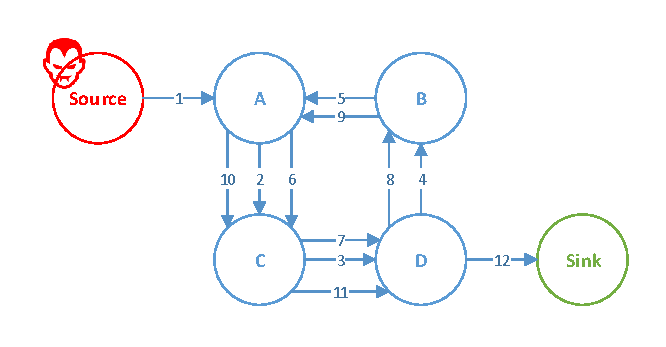
\includegraphics[width=0.9\linewidth]{figures/Carousel_Attack.pdf}
  \caption{Carousel Attack.}
  \label{fig:carousel_attack}
\end{figure}

\subsection{Stateful Protocols}
\label{sec:tables_routing}
In systems that use this type of routing protocols, network nodes are aware of the network topology and its state, being able to make local decisions on the node to whom they will forward the packet. The effect of the Vampires on this type of routing is limited since the route is built dynamically from many independent forwarding decisions. However, attackers can still cause damage by forcing packet forwarding through nodes that would not be on the optimal path, for example, by forwarding the packet back to the source. The Directional Antenna Attack is an example of such attacks. In this attack, the attacker takes the role of an intermediary and not the source of a packet. If the attacker has the resources to use a directional antenna, it can deposit a packet on arbitrary parts of the network while also forwarding the packet locally. This causes nodes that were not on the optimal path to also consume energy by forwarding a packet they would not normally receive, therefore increasing the total energy consumption by a factor of the directions the attacker can position the antenna and the distance between the receiver and the sink. Figure \ref{fig:directional_antenna_attack} shows an example where a ``vampire'' intermediary deposited a node on a distant location of the network, causing the packet to follow two different routes towards its destination

\begin{figure}[h]
  \centering
  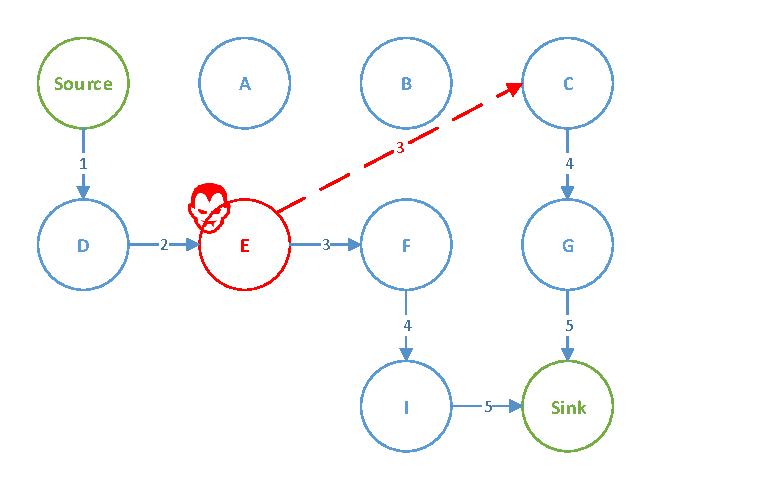
\includegraphics[width=0.8\linewidth]{figures/Directional_Antenna_Attack.pdf}
  \caption{Directional Antenna Attack.}
  \label{fig:directional_antenna_attack}
\end{figure}

While it is true that there are mitigation strategies available for these attacks, those strategies imply that additional checks and validations are performed on the network nodes. For example, nodes could check the packet headers for loops in the message path, and if found, update the route or simply drop the packet, therefore mitigating the carousel attack. If we were to mitigate the directional antenna attack, we could for example analyse the route paths of a given packet that reached the sink more than once. The last node identifier to appear duplicated before the path started to diverge would be the one who directed the packet to multiple regions, therefore revealing the attacker. Unfortunately, these mitigation strategies are placing a burden on the already constrained nodes. For each new attack that we wish to mitigate, additional checks and validations must be performed, eventually reaching a point were the costs involved in validating each packet could be considered an attack on the node resources. In order to address this issue, we propose that a secure bootstrapping is performed for every device that joins the network. The following section explains what is bootstrapping, how can it be performed and some existing solutions that follow this approach.

\section{Secure Bootstrapping}
\label{sec:secure_bootstrapping}
The term bootstrapping is applied to the process in which a new device is connected to an existing network. To achieve a secure bootstrapping, a unique identity and security parameters are associated with the device before this phase. There are several ways to carry out the initial setup, either via a physical interface or wirelessly. In the case of wireless bootstrapping, attention must be given to eavesdropping so that the secure credentials cannot be intercepted.Since the presented vampire attacks are to be performed by a malicious intruder capable of interacting with the network, if we could assure a secure bootstrapping, meaning that the new node would be authenticated before becoming an active member of the network, those attacks could no longer be performed.

Secure bootstrapping and network admission solutions have already been proposed in past literature. However, the development and optimization of application layer protocols as well as network layer routing schemes allows for new approaches and solutions that can now fit the nature of \gls{IoT} devices.
Bergman et al.\cite{Bergmann2012} proposed a three-phase secure bootstrapping technique for nodes in a \gls{CoAP} network. Firstly the joining node broadcasts a request for a \gls{CSDS}. This server, once contacted by a new node takes the responsibility of key distribution. Then the system goes under a vulnerable phase where the secret is transmitted from the \gls{CSDS} onto the new device. The author's proposes a short audible or visual feedback to the human installer when the secret is received and assumes that potential eavesdroppers can not intercept this transmission. Finally, this secret is used to setup the \gls{DTLS} connection. This approach has major security drawbacks on the secret transmission phase, so the authors propose limiting the radio power to a low level and disable data forwarding beyond the local network segment, but these techniques cannot assure that an attacker won't be able to intercept the transmission.\\
Oliveira et al. \cite{Oliveira2013} proposed an admission control solution for 6LoWPAN networks based on administrative approval. Each joining node would broadcast its presence to the network, and that broadcast would be received by the administrator in the management server. Then, the administrator would grant access to that new device based on its address, and that information would be transmitted to all the devices in the network. After this phase, the device would be allowed communication as a regular member of the network by its neighbours. This approach has the advantage of requiring no previous setup on the device before operation but is vulnerable to spoofing attacks \gls{ACL}. The authors state that work still needs to be performed in order to validate the sensor identity and leave as possibility the pre-instalment of keys on the device. 

Besides these related work efforts, there are additional secure bootstrapping techniques \cite{Fischer2012} that rely on tokens and one-time-passwords for cyphering the first communications and receiving security credentials, or even approaches where the manufacturers deploy those security credentials during the manufacturing process of the device vendor. Still these approaches either require additional hardware to be employed or the need to trust the manufacturer credentials.\\
In our work, we propose a secure bootstrapping method where:
\begin{itemize}
	\item No additional hardware needs to be employed during the bootstrapping process.
	\item No additional security credentials need to be fetched after the deploy on the field. 
	\item No security credentials need to be generated and uploaded to the joining nodes by third parties.
	\item No initial message exchange is sent unencrypted and/or unauthenticated.
\end{itemize}

In the following section, our complete proposed infrastructure is presented in terms of objectives and requirements, architecture, used protocols and implementations details. 

\section{Proposed Infrastructure}
\label{sec:proposed_infrastructure}
The \gls{IoT} principle of connecting every device do one another in an automated way can create networks beneficial to a wide spectrum of applications, ranging from home environments to large enterprises or even cities. However these are domains that have different requirements. A home application should be easy to setup without complex configurations. An enterprise solution can benefit from additional administrative configurations as long as the deployment of the network nodes is done quickly due to their potential large number. In order to demonstrate the capacities and applicability domain of our system, we will use a Smart University Campus scenario since it is out believe that it can effectively demonstrate the needs targeted by our work.
In the following sections we will apply the information gathered in terms of attacks and mitigation strategies to find suitable communication protocols and define our objectives and requirements. Then, a model of a university campus with our proposed power-efficient network architecture will be presented and their components role explained.


\subsection{Objectives and Requirements}
A major concern amongst \gls{IoT} application is the communication model. It is out goal that the entire network is power-aware, using the minimum energy possible. Also, it is very important that the deployment of new nodes and system maintenance can be performed by regular staff members without knowledge of the inner workings of the system. This creates usability challenges and requires simple and automated interfaces and bootstrapping processes. Additionally, the following set of requirements is critical in order to allow secure communications to take place.
\begin{itemize}
	\item Confidentiality: Without confidential message transmission, packets would flow in the network in plain text. Attackers could sniff the packets in order to obtain network activity information constituting a breach in security. Even if there is no critical data being sent, privacy is still compromised.
	\item Integrity: Assuring message integrity means that the message was not modified between the source and its destination. Without integrity we could not rely on the received data since it could have been, intentionally or not, modified on the fly, and be providing the system wrong information.
	\item Authentication: The studied type of networks relies on hop-to-hop communication, meaning several nodes will take place in forwarding a packet. If they are not authenticated they could perform a wide range of attacks and disrupt the network.
\end{itemize}

\subsection{Protocol Stack}
\label{sec:protocol_stack}
There are many alternatives and some proposed standards when it comes to choosing a protocol stack for \gls{IoT} communications \cite{Al-Fuqaha2015} implying that a thorough analysis of the existing solutions is necessary to unveil the strong and weak points of each candidate.   

\subsubsection{Data Link and Physical Layer}
\label{sec:data_link}
The first requirement for the physical layer of the \gls{IoT} is the use of wireless radios. These should aim for simplicity, low-power and low-cost communications. While wireless communication is widespread and can be found from homes to airports, the type of radio commonly used, known as Wi-Fi \cite{IEEE2012}, uses a high amount of power causing concerns for battery life. IEEE 802.15.4 \cite{IEEEComputerSociety2011} on the other hand was created for \gls{LR-WPAN} and its specifications focus on low power consumption, low data rate, low cost and high message throughput make it a strong candidate for \gls{IoT} applications.

\subsubsection{Network Layer}
\label{sec:network_layer}
The \gls{IoT} vision and its massive deployment can only be achieved through the use of IPv6 \cite{Pickard2015}. However, physical layers more suitable for communication over constrained networks pose some limitations to the use of the IPv6 messages. For example, the limited packet size in IEEE 802.15.4 based networks. To tackle these issues, the \gls{IETF} \gls{6LoWPAN} \cite{Shelby2012} working group developed a standard based on header compression to reduce the transmission overhead, fragmentation to meet the IPv6 \gls{MTU} requirements and forwarding to link-layer to support multi-hop delivery \cite{Hui2008}. \gls{6LoWPAN} is able to remove a major share of IPv6 overheads, being able to compress its headers to two bytes, therefore allowing small IPv6 datagrams to be sent over IEEE 802.15.4 networks. \\
With the use of 6LoWPAN, routing protocols can now use the IPv6 addressing scheme. Given the possible frequent topology changes associated with the radio-link instability, successful  solutions must take these requirements into account on their specification. \gls{RPL} \cite{Winter2012} can support a wide variety of link-layers and is prepared for devices with very limited resources. It is able to build up network routes, distribute routing knowledge among nodes and adapt the topology in a very efficient way. Furthermore, \gls{RPL} has a built in topology repair mechanism that acts in the case of a routing topology failure, link failure or node failure.

\subsubsection{Application Layer}
\gls{CoAP} \cite{Shelby2014} is a document transfer protocol based on \gls{REST} on top of \gls{HTTP} functionalities. \gls{CoAP} objective is to enable tiny constrained devices to use RESTful interactions, where clients and servers expose and consume web services using \gls{URIs} together with  \gls{HTTP} Get, Post, Put and Delete methods. Unlike \gls{REST}, \gls{CoAP} runs over \gls{UDP} instead of \gls{TCP} which makes it suitable for full IP networking in small micro-controllers. Retries and reordering are implemented at the application stack using a messaging sub-layer that detects duplicated messages and provides reliable communication using different types of messages. Confirmable messages must be acknowledged by the receiver, nonconfirmable follow the fire-and-forget model. Despite being a lightweight protocol, \gls{CoAP} still provides important features:
	
\begin{itemize}
	\item Resource Observation - \gls{CoAP} can extend the \gls{HTTP} request model with the ability to observe a resource therefore monitoring resources of interest using a publish/subscribe mechanism;
	\item Resource Discovery - \gls{CoAP} servers provide a list of resources using well-known {URIs} that allow clients to discover what resources are provided and their types;
	\item Interoperability - since \gls{CoAP} is based on the \gls{REST} architecture, a simple proxy enables \gls{CoAP} to easily interoperate with \gls{HTTP}.
\end{itemize}

A final overview of the presented stack for \gls{IoT} communication is presented in Table \ref{tab:stack} with the objective of comparing it to the protocol stack commonly used in the Internet.

\begin{table}[h]
	\centering
	\begin{center} \caption{Protocol Stack Comparison Overview } \label{tab:stack}\end{center}
	\begin{tabular}{c|c|c}
		Layer & Web & IoT \\
		\hline
		Application & \gls{HTTP} & \gls{CoAP} \\
		Transport & \gls{TCP} & \gls{UDP} \\
		Network & IPv6 & 6LoWPAN \\
		Data-Link/Physical & 802.11 & 802.15.4
	\end{tabular}
\end{table}

\subsection{System Architecture}
\label{sec:system_architecture}
As previously stated, we will use a Smart Campus scenario. Being aware of the technological improvements on sensor networks and building management technologies, the campus administration decided to improve the monitoring of the overall conditions of the buildings and inside environments in order to better preserve its assets. To cope with the new requirements, we propose a solution for the monitoring of the campus sections by deploying a wireless sensor network on each building, connected to a central management station operated by the available staff. The scenario will be based on the \gls{IST} campus model. An overview of the system and its components over the \gls{IST} blueprints can be found in Figure \ref{fig:global_architecture}. Regarding each individual component:

\begin{itemize}
	\item Numeric Nodes: Represent the network sensor nodes, the most constrained element of the network. They cooperate to build the topology and route messages hop-by-hop until the root is reached. These are fully equipped with the previously presented energy efficient protocol stack
	\item Alphabetical Nodes: Represent the root node of each section network topology. They are equipped with the same stack of the numbered nodes but are more powerful, preferentially not battery powered and act as the bridge between the constrained 6LoWPAN environment and the central management station. These nodes must be more powerful than the numeric ones so that they can process all the requests between a group of sensors and the management station. Also, although the numeric nodes use low-power wireless radios, the alphabetical nodes must be capable of interfacing with more power hungry radios and protocols therefore requiring more resources. This differentiation allows numeric nodes (the large portion of the network devices) to keep their very constrained nature, consuming less energy, an still be able to communicate with external devices.
	\item Management Station: A black box model of the core components of the system. Each building reports to the central station and the staff monitors the network status through it. A white box model will be shown in the following sections.
	\item Client: The system's clients can be any user with access credentials, but mostly the staff members. They can access the management station either from within the local network or from outside through the Internet.
\end{itemize}
 
\begin{figure}[h]
  \centering
  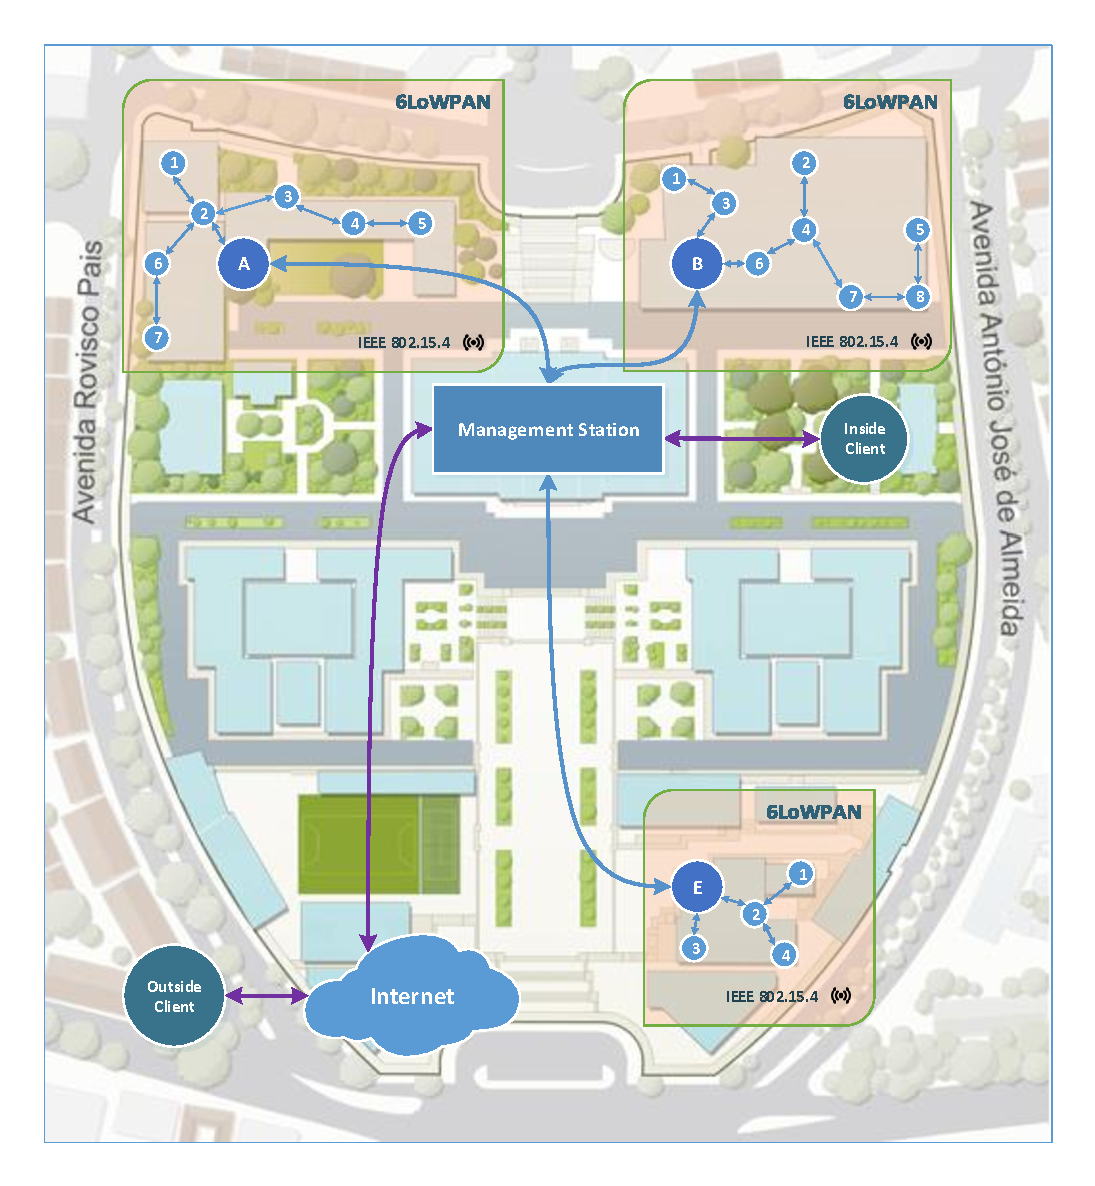
\includegraphics[width=1\linewidth]{figures/Global_Architecture.pdf}
  \caption{Global System Architecture}
  \label{fig:global_architecture}
\end{figure}

\paragraph{\textbf{Central Management Station}}
The central management station is divided in five main components. A white box schematic of the core components and interactions can be found in Figure \ref{fig:core_components}. Regarding each individual component:

\begin{itemize}
	\item Key Store: This component is responsible for storing the shared network key for the RPL protocol;
	\item Bootstrapper: The bootstrapper acts as the interface between the management station and the network devices. It generates the device identifier and writes it together with the shared network key into the new device;
	\item CoAP Client Observer:  The one and only client in the network. Instead of the user directly requesting the sensor readings, the client will observe each resource and be notified of the new value. Each time it receives an update, it stores the information on the Data Server for the clients to use;
	\item Data Server: A database with mappings of each node to the most up to date value reported. It's updated by the client observer and used on demand by the clients;
	\item Proxy: Responsible for bridging requests coming from the Internet to the Data Server. Responsible for authenticating the external clients and providing access to the Data Server information.
\end{itemize}

Although each user could access the system through a \gls{CoAP} terminal and request the most up-to-date readings from the sensor nodes, this approach would cause unnecessary overheads in the system. Since many clients can connect from different locations, many requests would be performed to the sensor nodes for the same information, this would mean additional memory usage in the physical devices, and more requests to the already constrained battery operated network. With the single client approach acting as an observer, only one message needs to go through the network for each new reading.

\begin{figure}[h]
  \centering
  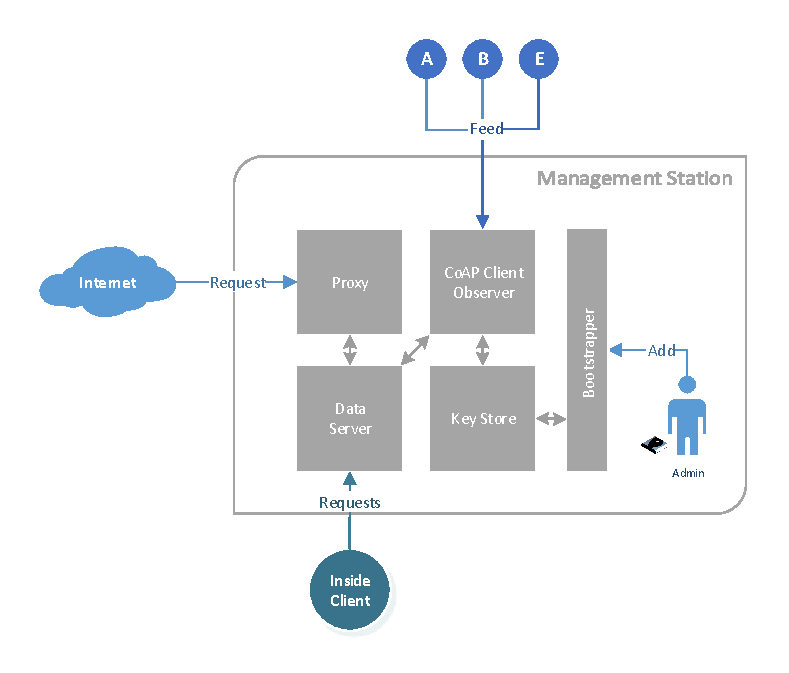
\includegraphics[width=1.05\linewidth]{figures/White_Box_Model.pdf}
  \caption{Central Management Station}
  \label{fig:core_components}
\end{figure}

\subsection{Implementation Details}
\label{sec:implementation_details}

NEW SECTION - TODO
o que faz o bootstrapper, que tecnologias usa (footnote para o github)\\
como é construido o cliente (californium e link para ele)\\
qual o sistema operativo escolhido e porque?\\
qual é o border router e o que usa?\\

Firstly, a software based approach was used to determine which hardware core components consumed most resources. An implementation of Energest\cite{Dunkels2007} for Contiki was selected since the tool maintains a table with entries for all components, such as CPU, radio transceiver, and LEDs. When a component starts running, a counter starts measuring the clock cycles used for that operation. When the component is turned off, the timer is stopped indicating how much resources were spent during that time.

A sensor node from the selected hardware type, with a baseline of the selected stack without any additional security measurements or optimizations was left working for 60 minutes while producing resource update messages every 60 seconds. The resource division, as obtained from Energest is presented in Figure \ref{fig:resource_alloc}.
%\vfill\break

\begin{figure}
\centering
\begin{tikzpicture}
[
    pie chart,
    slice type={comet}{blu},
    slice type={legno}{rosso},
    slice type={coltello}{giallo},
    slice type={sedia}{viola},
    slice type={caffe}{verde},
    pie values/.style={font={\small}},
    scale=2
]

    \pie{}{0.7/sedia,50.6/comet,0.1/legno,48.6/coltello}

    \legend[shift={(-1cm,-1cm)}]{{CPU (0.7\%)}/sedia, {LPM (50.6\%)}/comet}
    \legend[shift={(0.5cm,-1cm)}]{{Tx (0.1\%)}/sedia, {Rx (48.6\%)}/coltello}

\end{tikzpicture}
\caption{Resource Allocation} \label{fig:resource_alloc}
\end{figure}

We can see from the tool output that nearly half of the node resources is spent on radio activity. This is due to the fact, that out of the box, Contiki-OS uses a \gls{RDC} protocol that keeps the radio always turned on listening to inbound network transmissions. In the attempt to reduce this radio usage, the ContikiMAC\cite{Dunkels2011} \gls{RDC} protocol, also implemented in Contiki-OS was used.
This protocol reduces power consumption by turning the radio off and regularly turning it on to listen to network activity and receive inbound packages. After this phase, the radio is turned off again. With ContikiMAC, nodes can take part in network communication and keep their radios turned off for roughly 99\% of the time\cite{Dunkels2011}. The drawback are increased latency and decreased throughput due to the cost of keep retransmitting packets until the receiver turns its radio on.


\section{Evaluation}
\label{sec:evaluation}
In this section we measure and profile the resources required for the system operation in order to discover if our choice of protocols and mitigation strategies is suitable for \gls{IoT} hardware. This ranges from the memory required for the nodes operating system and protocol stack, to the hardware power consumptions. Furthermore we evaluate our bootstrapping infrastructure by measuring the time required for uploading a firmware to the new device and the ease of use by counting the steps required for the process to take place. Each following subsection both presents the collected data and explains the process and technologies involved in obtaining it.

\subsection{Hardware Suitability}
In order to evaluate if the \gls{IoT} hardware is capable of supporting our choice for the stack of protocols security measurements it is necessary to measure the firmware size. For that task, the \textit{msp430-size}\footnote{http://www.ti.com/tool/msp430-gcc-opensource} tool was used. This tool analyses the firmware file and outputs the amount of \textit{text}, \textit{data} and \textit{bss}.
\textit{Text} corresponds to code and constants, \textit{data} is for initialized variables and \textit{bss} is for uninitialized data (which is initialized with zero in the startup code).
The total amount of flash memory can be calculated from the sum of the text and data parameters.
The total amount of ram memory can be calculated from the sum of the data and bss parameters.
Both the firmware without security mechanisms and the one with link-layer security were analysed for their Flash and RAM usage. The results can be found in Table \ref{tab:space_req}. The inclusion of link-layer security represents a 3.02\% increase in Flash usage and a 1.02\% increase in RAM usage.

\begin{table}
\centering
\caption{Memory Usage}
\label{tab:space_req}
\begin{tabular}{|c|c|c|} \hline
Security Mechanism&Flash(KB)&RAM(KB)\\ \hline
No-Sec& 59.56& 13.54\\ \hline
LLSec& 61.36& 13.80\\ %\hline
%DTLS& 84.38 & 15.66\\ \hline
%LLSec and DTLS& 86.18& 15.91\\
\hline\end{tabular}
\end{table}

%\begin{figure}
%\centering
%\begin{tikzpicture}
%\begin{axis}[
%    symbolic x coords={NoSec, LLSec, DTLS, FullSec, cenas},
%	ylabel=Memory(KB), 
%	enlargelimits=0.05,
%	legend style={at={(0.5,-0.1)},
%	anchor=north,legend columns=-1},
%	ybar interval=0.8,
%]
%\addplot 
%	coordinates {(NoSec,59.96) (LLSec,61.36)
%		 (DTLS,84.38) (FullSec,86.18) (cenas,61.36)};
%\addplot 
%	coordinates {(NoSec,13.54) (LLSec,13.80) 
%		(DTLS,15.66) (FullSec,15.91) (cenas, 15.8)};
%\legend{Flash,RAM}
%\end{axis}
%\end{tikzpicture}
%\caption{Memory Occupation} \label{fig:space_req}
%\end{figure}

In order to be considered an \gls{IoT} capable device for this work, the selected hardware should possess a 802.15.4 radio, be capable of being battery powered and provide development tools like sensors and actuators that would be mapped to the application layer endpoints. The board also needs to be compatible with the selected operating system and provide low-power modes of operation. With all this in consideration, the Zolertia RE-Mote\footnote{http://zolertia.io/product/hardware/re-mote} board was selected since it fulfilled all the requirements and also provided an integrated cryptoprocessor while maintaining a low-power operation.
On the other hand, to assure our firmware size is a proper fit for current \gls{IoT} hardware we not only verified that if fits the Zolertia RE-Mote memory but also compared it to two other boards also designed for \gls{IoT} applications. The boards are the Arago Systems Wismote\footnote{http://www.wismote.com} and the Texas Instruments CC2538DK\footnote{http://http://www.ti.com/tool/cc2538dk}. The device's memory is shown in Table \ref{tab:hardware_memory} and allows us to conclude that our solution if practical for the target hardware.

\begin{table}
\centering
\caption{Hardware Memory}
\label{tab:hardware_memory}
\begin{tabular}{|c|c|c|} \hline
Device Name&Flash(KB)&RAM(KB)\\ \hline
Zolertia RE-Mote& 512& 32\\ \hline
Arago Systems Wismote& 128& 16\\ \hline
Texas Instruments CC2538DK& 512 & 32\\
\hline\end{tabular}
\end{table}

\subsection{Power Consumption}
The introduction of security mechanisms in low-power networks is necessary and desirable, however due to the low-power characteristics of \gls{IoT} sensor and actuator networks, a substantial increase in power consumption can disrupt the network by quickly draining the available resources. To this extent, a power consumption analysis was performed on our selected board in order to determine the most suitable battery powering solution. We performed current measurements during periods of silence as well as during periods of radio activity and calculated the power consumption in Watts(W) from the equation \ref{eq:power}, where I is the current in Amperes(A) and V is the voltage in Volts(V) as presented in Table \ref{tab:power_consumptions}.
\begin{equation}
\label{eq:power}
P = I  V
\end{equation} 

\begin{table}
\centering
\caption{Power Consumption}
\label{tab:power_consumptions}
\begin{tabular}{|c|c|c|c|} \hline
Mode&Voltage(V)&Current(mA)&Power(W)\\ \hline
Radio ON& 9.0& 17&0.15\\ \hline
Radio OFF& 9.0& 5.2&0.05\\ 
\hline\end{tabular}
\end{table}

Remembering that the ContikiMAC \gls{RDC} protocol allows to keep the radio turned off for roughly 99\% of the time\cite{Dunkels2011} the collected data shows that our solution maintains the low-power consumptions required for \gls{IoT} environments.

\subsection{Bootstrapping Process}
In order to evaluate our bootstrapping process we conducted an experiment on the amount of time (in seconds) required to bootstrap a new node as an indicator of the process efficiency. The process starts with the operator connecting the new device to the bootstrapper and finishes with the operator removing the device from the bootstrapper. During the process the operator needs to open the user interface, select the appropriate device and press the upload button. In the background the system will compile the source code to match the target platform, then it will erase the previous firmware and finally upload the new one. The experiments result are presented in Table \ref{tab:bootstrapping_time}. Although the apparent bootstrapping process time is xx seconds, the process efficiency is especially important when bootstrapping multiple devices. In this case, after the first one, the user interface and target hardware will already be open and selected and the source code will already be compiled, resulting in a real time of xx seconds. If needed, an operator could perform xx bootstrapping processes in a single hour, so we can conclude that our solution if practical for the presented scenario.

\begin{table}
\centering
\caption{Bootstrapping Timings}
\label{tab:bootstrapping_time}
\begin{tabular}{|c|c|} \hline
Operation&Time(s)\\ \hline
Insert New Device&1\\ \hline
Open User Interface&4\\ \hline
Select Target Hardware&2\\ \hline
Compile Source Code&xx\\ \hline
Erase Previous Firmware&xx\\ \hline
Upload New Firmware&xx\\ \hline
Remove New Device&x\\ 
\hline\end{tabular}
\end{table}


\section{Conclusions}
\label{sec:conclusion}
Due to the limitations of \gls{IoT} devices, achieving secure communications is not an easy task. In order to allow the deployment of battery powered nodes, their communication model must be very efficient and consume the minimum amount of power required for operation. To achieve those requirements we started by analysing the existing protocols across the OSI layers, trying to find the best suited solutions for this type of environments. After a thorough comparison we achieved a working stack of protocols but soon discovered possible breaches and attacks, especially on the network layer. Those attacks were further investigated and catalogued. Given the common principle on the majority of the attacks, the introduction of rogue nodes to the network, we presented some possible solutions based on secure bootstrapping, the secure authentication of new nodes when joining a network.
Once the energy efficient stack, possible attacks and mitigation strategies were defined, we proposed our solution based on a Smart Campus scenario. This solution is focused on providing the joining devices all the secure credentials required for a secure bootstrapping before the deploy on the field, so that when they start the operation phase no additional credentials need to be fetched, implying that no additional energy is spent on configuration.
Always maintaining a power-aware perspective, the system has been evaluated by measuring its energy consumption with different configurations and core battery usage components. This charting allows future users of the system to decide the type of resources they need to allocate in order to achieve a desired level of security for their application.
As future work, memory access protection should be addressed in order to prevent the stealing of secure credentials from deployed devices.
%\end{document}  % This is where a 'short' article might terminate

%ACKNOWLEDGMENTS are optional
%\section{Acknowledgments}
%This section is optional; it is a location for you
%to acknowledge grants, funding, editing assistance and
%what have you.  In the present case, for example, the
%authors would like to thank Gerald Murray of ACM for
%his help in codifying this \textit{Author's Guide}
%and the \textbf{.cls} and \textbf{.tex} files that it describes.

%
% The following two commands are all you need in the
% initial runs of your .tex file to
% produce the bibliography for the citations in your paper.
\bibliographystyle{abbrv}
\bibliography{sigproc}  % sigproc.bib is the name of the Bibliography in this case
% You must have a proper ".bib" file
%  and remember to run:
% latex bibtex latex latex
% to resolve all references
%
% ACM needs 'a single self-contained file'!
%
%APPENDICES are optional
%\balancecolumns
%\appendix
%Appendix A

\end{document}
